
\subsubsection{a)}

Consider the Poisson equation in 1D

\begin{equation}
\label{task5Poisson}
    -u_{xx} = f(x), \hspace{2mm} u(a) = d_1, \hspace{1mm} u(b) = d_2.
\end{equation}
Assume a uniform partition, i.e. that $x_m = a + mh$, $h = \frac{b-a}{M}$ and $m \in [0,M]$. By discretizing the problem with linear finite elements, a linear system $\mathbf{Au} = \mathbf{f}$ can be created. Since the problem has inhomogeneous Dirichlet boundary conditions, the approach outlined in section 2.5 of \cite{Curry} will be followed, in order to create the system.  
As is done in Curry's note, the inhomogeneous problem will be related to the homogeneous one. The weak form is therefore written with test functions satisfying $v \in H^1_0([a,b])$, i.e. $v(a) = v(b) =0$. The weak form becomes

\begin{align}
    -\int_a^bu''(x)v(x)\mathrm{d}x &= \int_a^bf(x)v(x)\mathrm{d}x, \nonumber \\
    \int_a^bu'(x)v'(x)\mathrm{d}x - [u'(x)v(x)]_a^b &= \int_a^bf(x)v(x)\mathrm{d}x, \nonumber \\
    \int_a^bu'(x)v'(x)\mathrm{d}x &= \int_a^bf(x)v(x)\mathrm{d}x,
    \label{var}
\end{align}

\noindent where $u$ is an element of $H^1([a,b])$. Next, $R_h \in H^1([1,b])$ is introduced, satisfying $R_h(a) = d_1$ and $R_h(b) = d_2$. Then $\hat{u} := u - R_h \in H^1_0([a,b])$ is defined, so the variational \eqref{var} form can be rewritten as 

\begin{equation}
    \int_a^b\hat{u}'(x)v'(x)\mathrm{d}x = \int_a^bf(x)v(x)\mathrm{d}x - \int_a^bR_h'(x) v'(x) \mathrm{d}x.
\label{var2}
\end{equation}

\noindent Using linear finite elements, the functions in \eqref{var2} are now restricted to lie in the finite dimensional subspace $X_h^1$ of $H^1([a,b])$, i.e. the space of piece-wise linear functions with basis $\{\varphi_i\}$ as defined in \cite{Curry}. We partition the grid into $M$ elements, such that $v = \sum_{i = 0}^{M}v_i \varphi_i(x)$ and likewise for $u$ and $\hat{u}$. $R_h$ takes the natural form $R_h = d_1 \varphi_0(x) + d_2 \varphi_M(x)$. Introducing the stiffness matrix $A_{ij} = \int_a^b \varphi'_i(x) \varphi'_j(x) \mathrm{d}x$  such that 

\begin{equation*}
    A =  \frac{1}{h}\begin{pmatrix}
        1 & -1 & 0 & \cdots & \cdots & 0 \\
        -1 & 2 & -1 & \ddots &   & \vdots \\
        0 & -1 & 2 & \ddots & \ddots & \vdots \\
        \vdots & \ddots & \ddots & \ddots & \ddots & 0 \\
        \vdots &  & \ddots & -1 & 2 & -1 \\
        0 & \cdots & \cdots & 0 & -1 & 1
    \end{pmatrix} \in \mathbb{R}^{(M+1) \times (M+1)},
\end{equation*}

\noindent and removing $v$, the equation \eqref{var2} becomes

\begin{equation}
\begin{split}
    A\hat{u} &= F-A(d_1, 0, \dots, 0, d_2)^T \\
             &= 
            \frac{1}{h}\begin{pmatrix}
                Q_0[(x_1 - x) f(x)] \\
                Q_0[(x - x_0) f(x)] + Q_1[(x_2 - x) f(x)] \\
                \vdots \\
                Q_{M-2}[(x - x_{M-2}) f(x)] + Q_{M-1}[(x_M - x) f(x)] \\
                Q_{M-1}[(x - x_{M-1}) f(x)]
            \end{pmatrix}
            -
            \frac{1}{h} \begin{pmatrix}
                d_1 \\
                -d_1 \\
                \vdots \\
                -d_2 \\
                d_2
            \end{pmatrix},
\label{task5system}
\end{split}
\end{equation}
where $Q_k[g(x)]$ denotes the Gaussian quadrature of the function $g$ over the interval $[x_k, x_{k + 1}]$. In the numerical implementation, we have use Gauss-Legendre quadrature with 5 sample points and weights. Then, the boundary conditions are implemented by removing the first and last row and column from the stiffness matrix $A$ on the left side of equation \eqref{task5system}, in addition to the first and last entries of the vector $F - A(d_1, \ldots, d_2)^T$. The resulting matrix and vector are given as

\begin{equation}
\begin{split}
    &\mathbf{A} :=  \frac{1}{h}\begin{pmatrix}
        -2 & -1 &  &  \\
        -1 & \ddots & \ddots &  \\
         & \ddots & \ddots & -1  \\
         &  & -1 & 2  \\
    \end{pmatrix} \in \mathbb{R}^{(M-1) \times (M-1)}, \\  \\
     &\mathbf{f} := 
    \begin{pmatrix}
                Q_0[(x - x_0) f(x)] + Q_1[(x_2 - x) f(x)]  + d_1/h\\
                \vdots \\
                Q_{M-2}[(x - x_{M-2}) f(x)] + Q_{M-1}[(x_M - x) f(x)] + d_2/h 
    \end{pmatrix} \in \mathbb{R}^{(M-1) \times 1},
\end{split}
\label{5a.system}
\end{equation}
respectively. Also, define $\mathbf{u} := \hat{u}$, so the system to be solved can be written as $\mathbf{Au} = \mathbf{f}$. Finally, when this system is solved, the vector $\hat{u}$ is expanded from dimension $M-1$ to $M+1$ by including $d_1$ as first entry and $d_2$ as the last, i.e. take $u(x) = \hat{u}(x) + R_h(x)$. 


\subsubsection{b)}
Now consider $0 \le x \le 1$ with 

\begin{equation}
    f(x) = -2, \quad d_1 = 0, \; d_2 = 1.
\label{5b}
\end{equation}
First, the analytical solution is calculated. The Poisson equation reads $-u_{xx} = -2$, which yields

\begin{equation}
    u(x) = x^2 + c_1x + c_2,
\end{equation}
where $c_1,c_2 \in \mathbb{R}$ are constants. The boundary conditions finally give $c_1 = c_2 = 0$, resulting in

\begin{equation}
    u(x) = x^2.
\end{equation}

When using the finite element method, both uniform mesh refinement (hereafter UFEM) and adaptive mesh refinement (hereafter AFEM) is performed. In the rest of the problem, when performing UFEM, $M = \{8,16,32,64,128,256,512,1024,2048\}$ will be used. On the contrary, AFEM will be performed using \textit{average}-error with $\alpha = 1$, and \textit{max}-error with $\alpha = 0.7$ as it is defined in section \ref{adaptive}.

Convergence plots, where the difference between analytical and numerical solution in $L_2$-norm is calculated, for both UFEM and AFEM are depicted in figure \ref{fig:5b}. It is apparent that all methods converge with order $\mathcal{O}(h^2)$ in $L_2$ norm. It can be shown that this is the expected theoretical result \cite{Curry}.

\begin{figure}[!t]
  \centering
  \subfloat[]{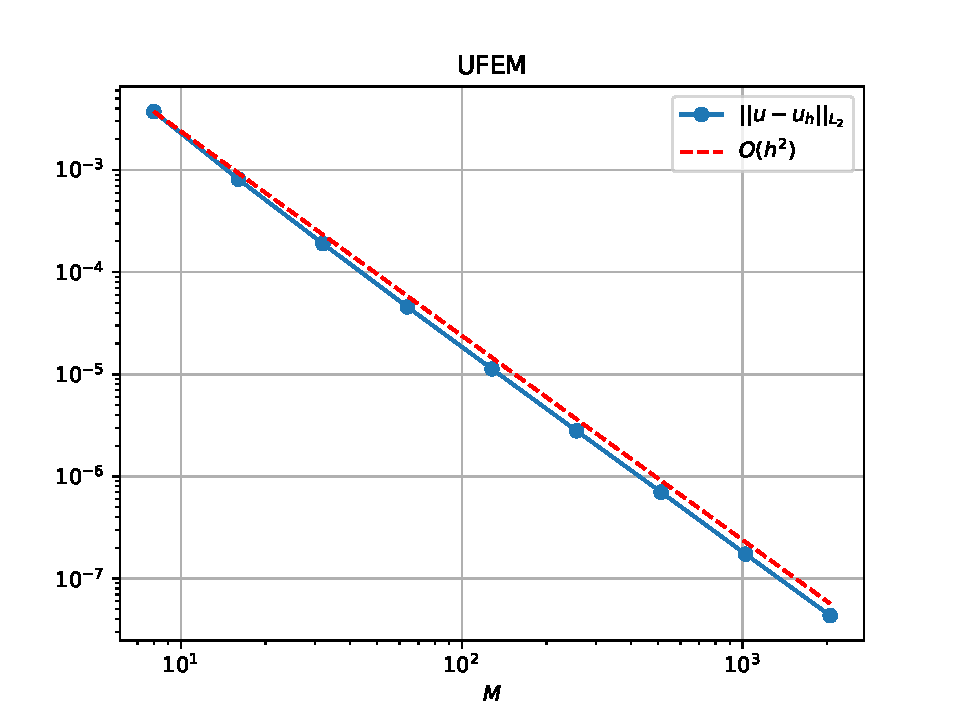
\includegraphics[width=0.5\textwidth]{plots/5b_UFEM.pdf}\label{fig:f1}}
  \hfill
  \subfloat[]{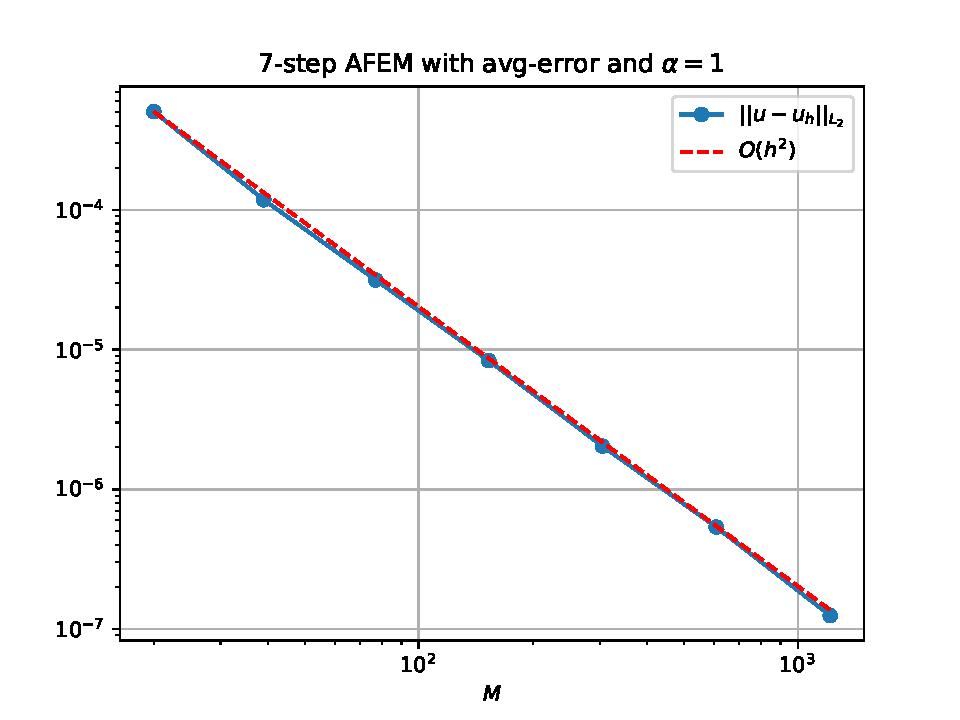
\includegraphics[width=0.5\textwidth]{plots/5b_avgAFEM.pdf}\label{fig:f2}}
  \hfill
  \subfloat[]{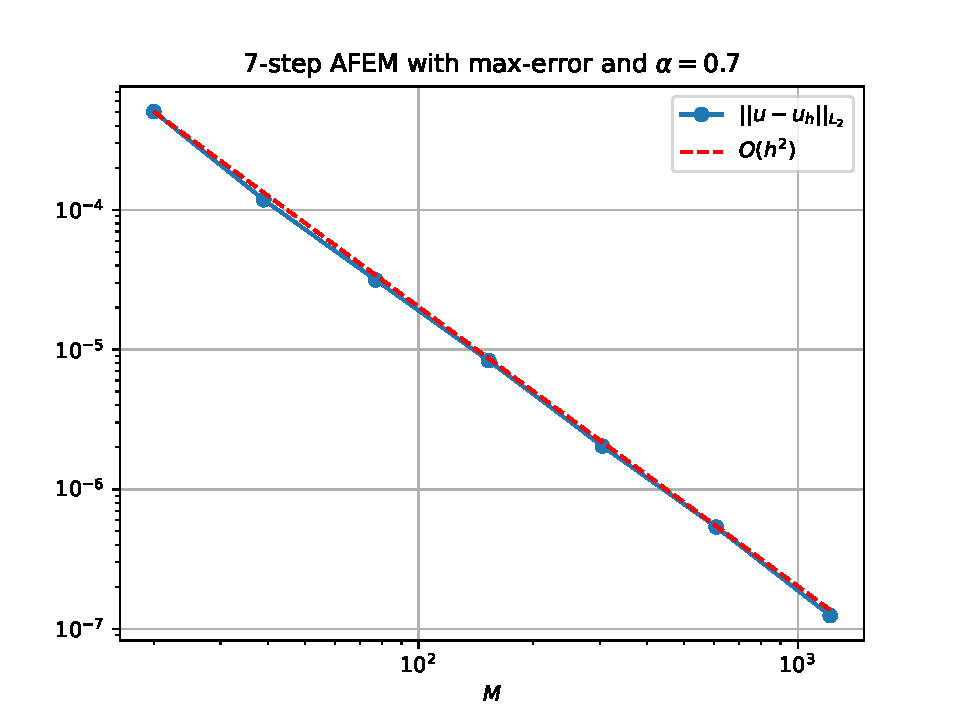
\includegraphics[width=0.5\textwidth]{plots/5b_maxAFEM.pdf}\label{fig:f3}}
  \caption{One dimensional Poisson equation $-u_{xx} = -2$ with $x \in [0,1]$ and $u(0) = 0, u(1) = 1$. The $L^2$-error is displayed in "log-log" plots. $u_h$ is the numerical solution while $u$ is the analytical solution. (a) UFEM. (b) AFEM with average-error and $\alpha = 1$. (c) AFEM with maximum-error and $\alpha = 0.7$.}
  \label{fig:5b}
\end{figure}

\subsubsection{c)}
Next, consider $-1 \le x \le 1$ with 

\begin{equation}
    f(x) = -(40000x^2-200)e^{-100x^2}, \quad d_1 = e^{-100}, \; d_2 = e^{-100}.
\label{5c}
\end{equation}
First, the analytical solution is calculated. The Poisson equation reads

\begin{equation}
    u_{xx} =  200e^{-100x^2} - 40000x^2 \cdot e^{-100x^2},
\end{equation}
which gives

\begin{equation}
    u(x) = e^{-100x^2} + c_1x + c_2
\end{equation}
The boundary conditions readily give that $c_1 = c_2 = 0$, which means the analytical solution is

\begin{equation}
u(x) = e^{-100x^2}.
\end{equation}

\noindent The convergence plots for UFEM and AFEM, in this case, are depicted in figure \ref{fig:5c}. It is apparent that all methods converge with order $\mathcal{O}(h^2)$ in $L_2$ norm.

\begin{figure}[!t]
  \centering
  \subfloat[]{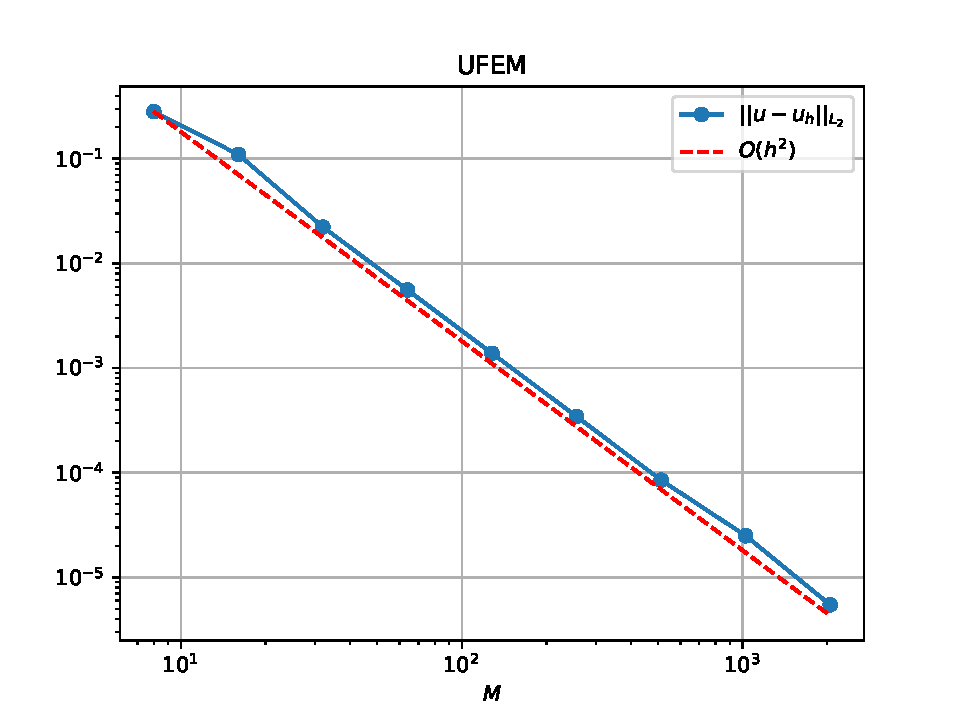
\includegraphics[width=0.5\textwidth]{plots/5c_UFEM.pdf}\label{fig:f1}}
  \hfill
  \subfloat[]{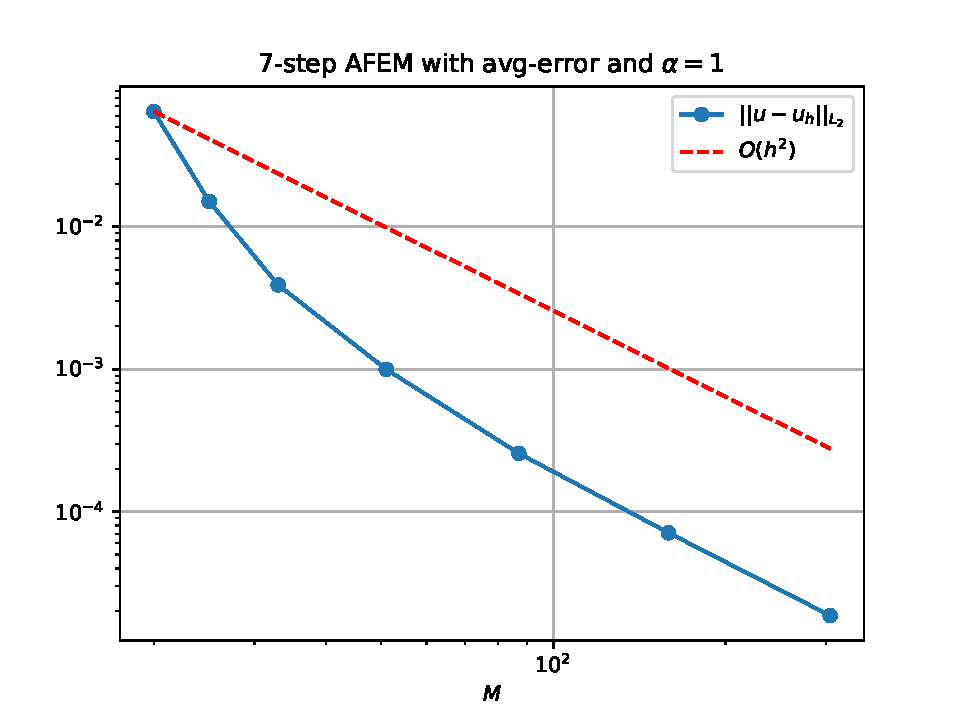
\includegraphics[width=0.5\textwidth]{plots/5c_avgAFEM.pdf}\label{fig:f2}}
  \hfill
  \subfloat[]{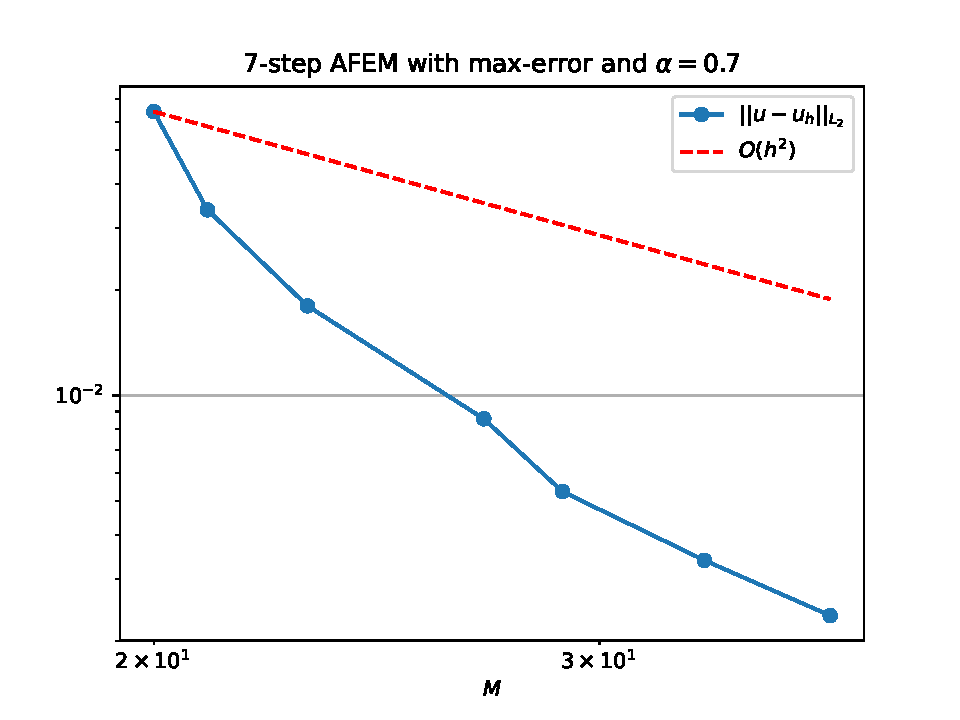
\includegraphics[width=0.5\textwidth]{plots/5c_maxAFEM.pdf}\label{fig:f3}}
  \caption{One dimensional Poisson equation $-u_{xx} = -(40000x^2 - 200)e^{-100x^2}$ with $x \in [-1,1]$ and $u(-1) = u(1) = e^{-100}$. The $L^2$-error is displayed in "log-log" plots. $u_h$ is the numerical solution while $u$ is the analytical solution. (a) UFEM. (b) AFEM with average and $\alpha = 1$. (c) AFEM with maximum and $\alpha = 0.7$.}
  \label{fig:5c}
\end{figure}

\subsubsection{d)}

Now consider $-1 \le x \le 1$ with

\begin{equation}
    f(x) = -(4000000x^2 - 2000)e^{-1000x^2}, \quad d_1 = e^{-1000}, \; d_2 = e^{-1000}.
\label{5d}
\end{equation}
\noindent The derivation of the analytical solution is entirely analogous the one in c). Thus,

\begin{equation}
    u(x) = e^{-1000x^2}.
\end{equation}

\noindent The convergence plots for UFEM and AFEM are depicted in figure \ref{fig:5d}. It is apparent that all methods converge with order of at least $\mathcal{O}(h^2)$ in $L_2$ norm.

\begin{figure}[!t]
  \centering
  \subfloat[]{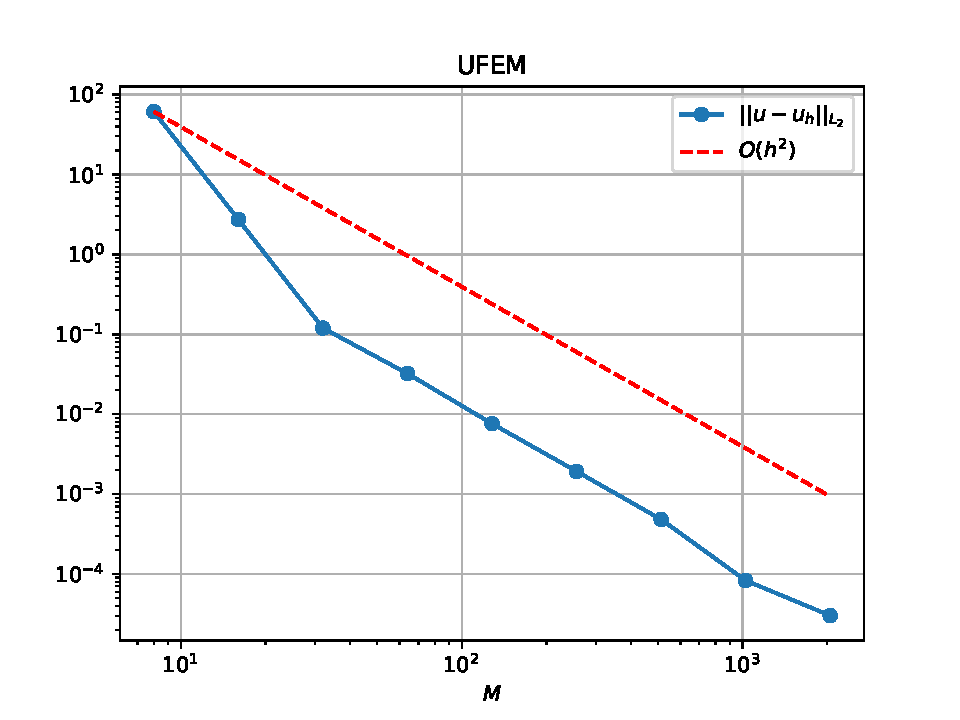
\includegraphics[width=0.5\textwidth]{plots/5d_UFEM.pdf}\label{fig:f1}}
  \hfill
  \subfloat[]{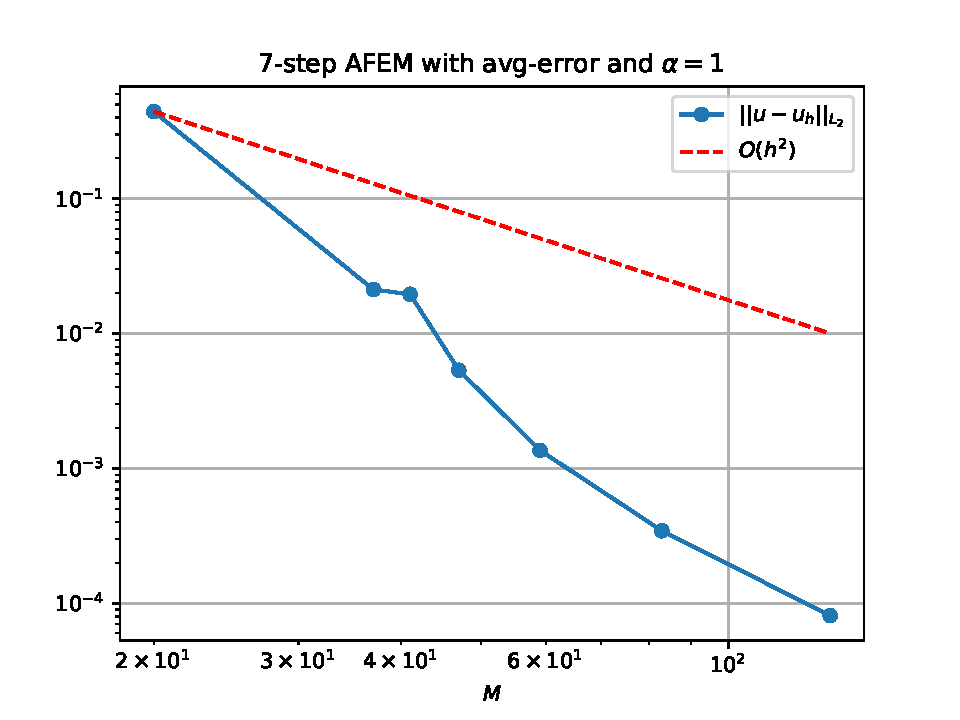
\includegraphics[width=0.5\textwidth]{plots/5d_avgAFEM.pdf}\label{fig:f2}}
  \hfill
  \subfloat[]{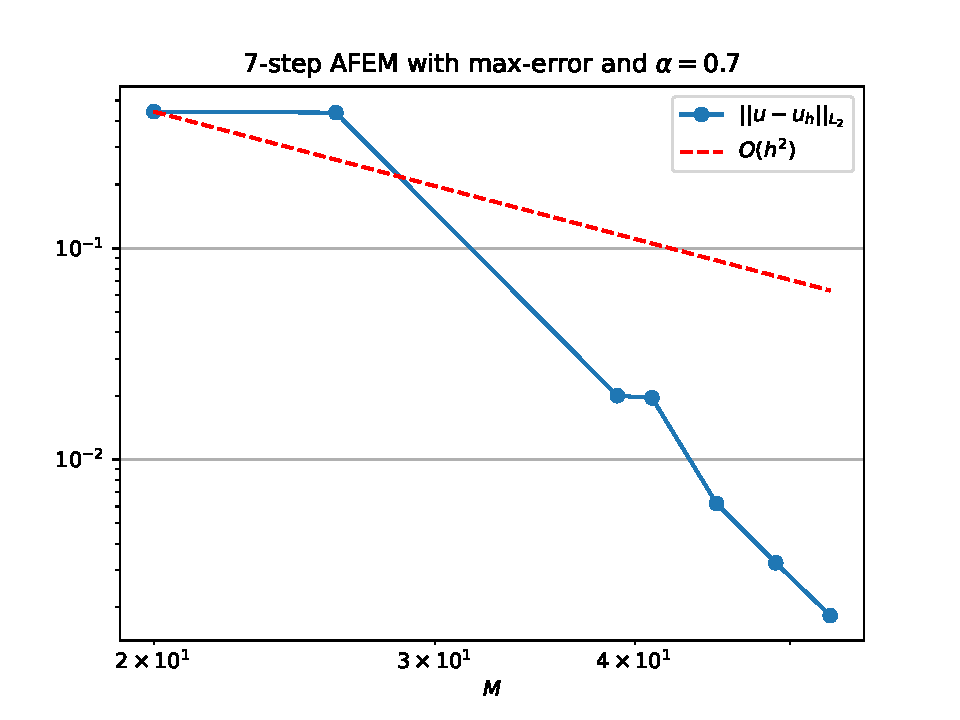
\includegraphics[width=0.5\textwidth]{plots/5d_maxAFEM.pdf}\label{fig:f3}}
  \caption{One dimensional Poisson equation $-u_{xx} = -(4000000x^2 - 2000)e^{-1000x^2}$ with $x \in [-1,1]$ and $u(-1) = u(1) = e^{-1000}$. The $L^2$-error is displayed in "log-log" plots. $u_h$ is the numerical solution while $u$ is the analytical solution. (a) UFEM. (b) AFEM with average and $\alpha = 1$. (c) AFEM with maximum and $\alpha = 0.7$.}
  \label{fig:5d}
\end{figure}

\subsubsection{e)}
Finally, consider $0 \le x \le 1$, with

\begin{equation}
    f(x) = \frac{2}{9}x^{-4/3}, \quad d_1 = 0, \; d_2 = 1
\label{5e}
\end{equation}
Integraiton yields that $u$ must be on the form $u(x) = x^{2/3} + c_1x + c_2$, where $c_1,c_2 \in \mathbb{R}$ are constants. The boundary conditions give $c_1 = 0$ and  $c_2 = 0$, so we arrive at the analytical solution

\begin{equation}
    u(x) = x^{2/3}.
\end{equation}

\noindent The convergence plots for UFEM and AFEM are depicted in figure \ref{fig:5e}. We observe that using uniform refinement only yields a convergence of order $\mathcal{O}(h)$ in this case. One possible explanation for this is that the analytical solution, $u(x)$ is not sufficiently smooth. For example, it is assumed that the variational, written as

\begin{equation}
    \int_0^1 u'(x) v'(x) \mathrm{d}x= \int_0^1 f(x)v(x) \mathrm{d}x
\label{varform}
\end{equation}

\noindent should hold for all $v \in H_0^1([0,1])$, where $v(0) = v(1) = 0$. If we let $v(x) = \sin(\pi x)$, the left hand side of \eqref{varform} becomes

\begin{equation}
\begin{split}
    \int_0^1 f(x)v(x) \mathrm{d}x &= \int_0^1 \frac{2}{9}x^{-\frac{4}{3}} \cdot \sin(\pi x) \mathrm{d}x \\
    &= \left[\frac{2}{9}x^{-\frac{4}{3}} \cdot (-\frac{1}{\pi}\cos(\pi x))\right]_0^1 - \int_0^1  \frac{8}{27} x^{-\frac{7}{3}} \cdot \frac{1}{\pi}\cos(\pi x) \mathrm{d}x,
\end{split}
\end{equation}

\noindent where it is readily seen that the first term is not defined for $x = 0$. The AFEM method with average error also seems to have a lower convergence rate compared to the other examples, while AFEM with max-error seems to uphold the convergence of rate $\mathcal{O}(h^2)$.

\begin{figure}[!t]
  \centering
  \subfloat[]{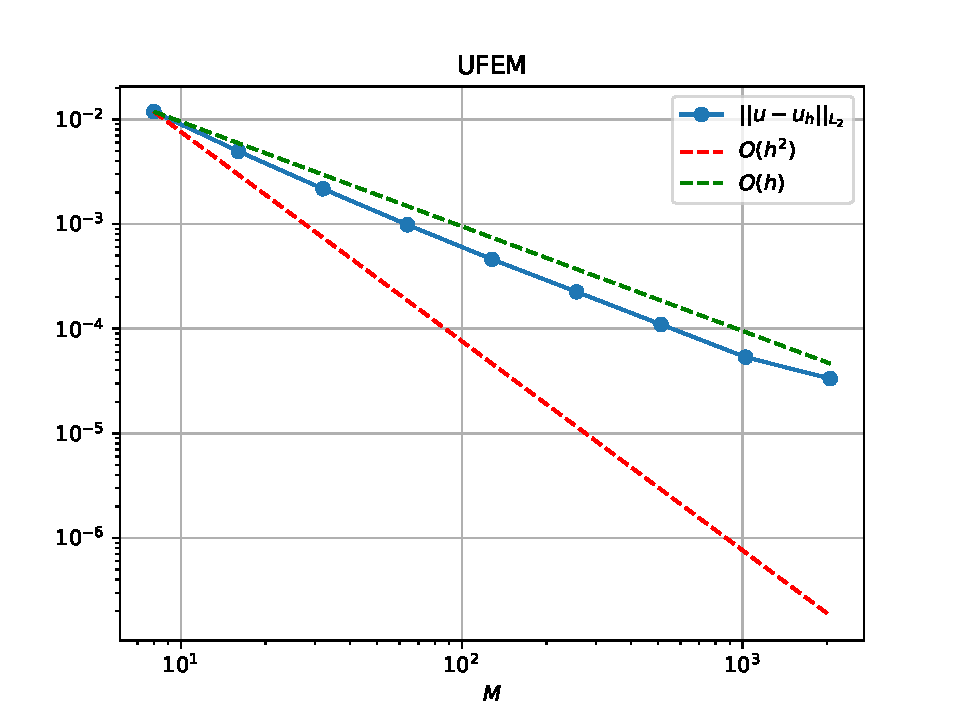
\includegraphics[width=0.5\textwidth]{plots/5e_UFEM.pdf}\label{fig:f1}}
  \hfill
  \subfloat[]{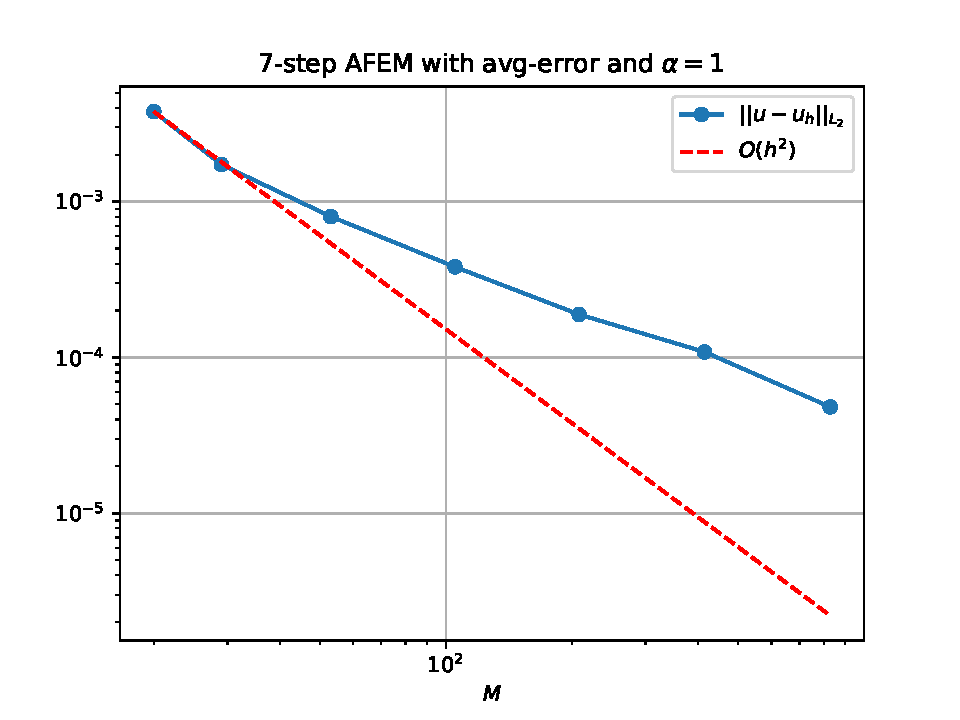
\includegraphics[width=0.5\textwidth]{plots/5e_avgAFEM.pdf}\label{fig:f2}}
  \hfill
  \subfloat[]{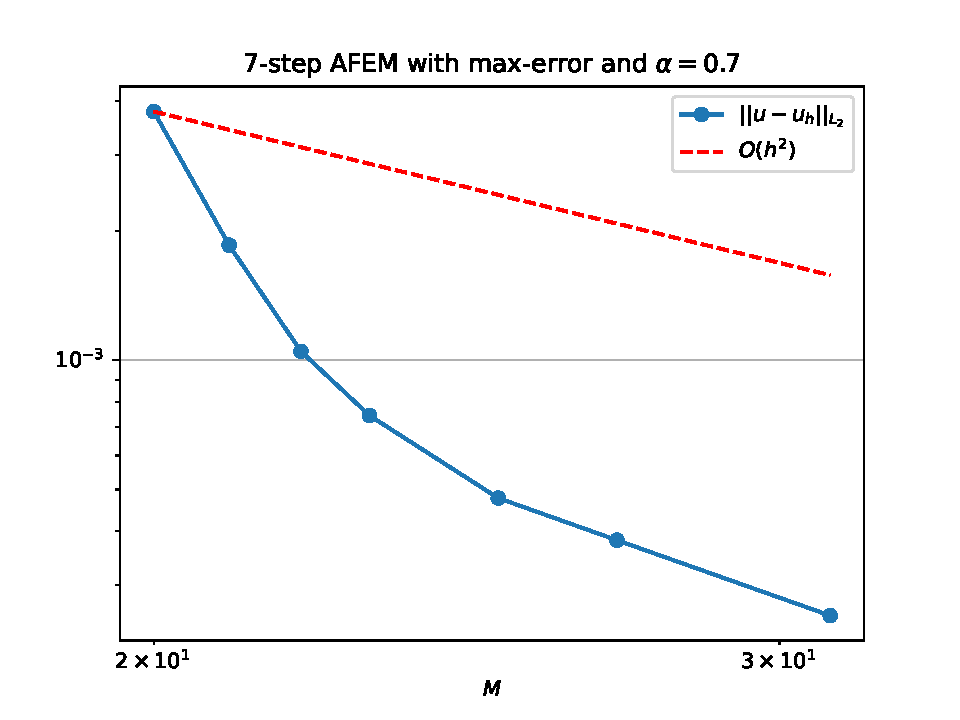
\includegraphics[width=0.5\textwidth]{plots/5e_maxAFEM.pdf}\label{fig:f3}}
  \caption{One dimensional Poisson equation $-u_{xx} = -\frac{2}{9}x^{-4/3}$ with $x \in [0,1]$ and $u(0) = 0,  u(1) = 1$. The $L^2$-error is displayed in "log-log" plots. $u_h$ is the numerical solution while $u$ is the analytical solution. (a) UFEM. (b) AFEM with average and $\alpha = 1$. (c) AFEM with maximum and $\alpha = 0.7$.}
  \label{fig:5e}
\end{figure}
\newpage
\ 
\newpage
